\documentclass[letterpaper]{article} % DO NOT CHANGE THIS
\usepackage{aaai2027}  % DO NOT CHANGE THIS
\usepackage[hyphens]{url}  % DO NOT CHANGE THIS
\usepackage{graphicx} % DO NOT CHANGE THIS
\urlstyle{rm} % DO NOT CHANGE THIS
\def\UrlFont{\rm}  % DO NOT CHANGE THIS
\usepackage{natbib}  % DO NOT CHANGE THIS AND DO NOT ADD ANY OPTIONS TO IT
\usepackage{caption} % DO NOT CHANGE THIS AND DO NOT ADD ANY OPTIONS TO IT
\frenchspacing  % DO NOT CHANGE THIS
\setlength{\pdfpagewidth}{8.5in} % DO NOT CHANGE THIS
\setlength{\pdfpageheight}{11in} % DO NOT CHANGE THIS

\usepackage[brazil]{babel}   % "Tabela", "Figura" e hifenização em português
\usepackage{booktabs}
\usepackage{amsmath}

\pdfinfo{
/TemplateVersion (2027.2)
}

\setcounter{secnumdepth}{0}

\title{Redes Neurais Artificiais para Classificação de Dígitos Manuscritos (MNIST)}
\author{
    Vinicius Pinho Galvão
}
\affiliations{
    Departamento de Ciência da Computação\\
    Universidade Federal de Minas Gerais\\
    viniciuspgalvao@dcc.ufmg.br
}

\begin{document}

\maketitle

% ---------------------------------------------------------------------------
\section{Introdução e Objetivo}
O MNIST reúne 70.000 imagens de 28$\times$28 pixels de dígitos manuscritos; reconhecê-los é um problema de classificação multiclasse com $C = 10$. Neste trabalho foi implementada do zero, em NumPy, uma RNA de duas camadas (uma escondida e uma de saída) treinada por gradiente descendente, com o objetivo de entender cada peça (propagação, ativações, perda e gradiente) e medir o efeito da taxa de aprendizado, do número de épocas e do número de neurônios. A melhor configuração ($\alpha = 0{,}5$, 256 neurônios, 500 épocas) atingiu 95,44\% de acurácia de teste. Na interface, porém, foi preciso aprender a desenhar com o centro de massa do dígito próximo ao das imagens do MNIST para que a rede acertasse.

% ---------------------------------------------------------------------------
\section{Metodologia}

\subsection{Dados e Arquitetura}
A função \texttt{load\_mnist} carrega o MNIST do OpenML, normaliza os pixels para $[0,1]$ (divisão por 255), divide os dados aleatoriamente em 80/20 (\texttt{random\_state} = 42), com 56.000 imagens de treino e 14.000 de teste, e codifica os rótulos em \emph{one-hot}. Cada imagem vira um vetor de 784 entradas, e as matrizes têm um exemplo por linha.

A rede tem 784 entradas, $H$ neurônios escondidos e 10 saídas. Os pesos $W_1$ ($784 \times H$) e $W_2$ ($H \times 10$) são inicializados com \texttt{np.random.randn}$\,\times\, 0{,}01$, e os vieses $b_1$ e $b_2$, com zeros. Pesos aleatórios quebram a simetria (neurônios iguais receberiam gradientes iguais e nunca se diferenciariam), e a escala pequena faz a rede começar perto da região linear das ativações, com perda inicial de $\ln 10 \approx 2{,}30$.

\subsection{Propagação e Funções de Ativação}
\begin{align*}
Z_1 &= X W_1 + b_1, & A_1 &= \mathrm{ReLU}(Z_1),\\
Z_2 &= A_1 W_2 + b_2, & A_2 &= \mathrm{softmax}(Z_2).
\end{align*}
$Z$ é a pré-ativação e $A$ a ativação; $b$ é somado a todas as linhas por \emph{broadcasting}. A ReLU, $\max(0, z)$, introduz a não linearidade: sem ela, as duas camadas colapsariam numa única transformação linear. O softmax, aplicado por linha, transforma os \emph{logits} em probabilidades que somam 1. Antes da exponencial, subtrai-se o máximo de cada linha: a constante se cancela no numerador e no denominador, mas evita estouro (sem ela, \texttt{softmax([1000, 1001, 1002])} devolvia \texttt{nan}).

\subsection{Função de Perda e Treinamento}
\[
L = -\frac{1}{m} \sum_{i=1}^{m} \sum_{c=1}^{C} y_{ic} \log \hat{y}_{ic}
\]
O \emph{one-hot} funciona como máscara: em cada exemplo só sobra o $-\log$ da probabilidade dada à classe certa, e a divisão por $m$ torna a perda comparável entre conjuntos de tamanhos diferentes. A versão vetorizada, com um único \texttt{np.sum}, foi cerca de 90 vezes mais rápida que a versão com laços (9\,ms contra 828\,ms com 56.000 exemplos).

O treino usa gradiente descendente em lote completo: a cada época, \texttt{forward}, perda, \texttt{backward} (fornecido) e $w \leftarrow w - \alpha\,\partial L / \partial w$. A acurácia compara o \texttt{argmax} por linha dos rótulos e das previsões. As funções foram validadas contra os resultados esperados do enunciado (seções 3.1 a 3.6).

\subsection{Protocolo Experimental}
Os treinos rodaram fora da interface, com um script auxiliar (\texttt{experiments/run\_experiments.py}) que repete o laço do \texttt{server.py}: um passo de gradiente no treino e a acurácia no teste a cada época. A semente 42 é fixada antes de cada inicialização, o que torna os treinos reproduzíveis e comparáveis. A busca é coordenada: o exp.~1 varia $\alpha$ com $H = 64$ e 500 épocas; a melhor taxa ($\alpha = 0{,}5$) fica fixa nos exp.~2 (varia $H$, 500 épocas) e~3 (varia as épocas, $H = 64$). Ambiente: AMD Ryzen 5 3600 (WSL2), Python 3.14.10, NumPy 2.3.5.

% ---------------------------------------------------------------------------
\section{Experimentos e Resultados}

\begin{table}[t]
\centering
\setlength{\tabcolsep}{5pt}
\begin{tabular}{lrrrr}
\toprule
 & Valor & Perda & Acurácia & Tempo (s) \\
\midrule
\multicolumn{5}{l}{\emph{Exp.\ 1: taxa de aprendizado} ($H = 64$, 500 épocas)} \\
 & 0,001 & 2,2997 & 14,91\% & 118 \\
 & 0,01  & 2,0891 & 45,19\% & 118 \\
 & 0,1   & 0,3417 & 90,21\% & 110 \\
 & 0,5   & 0,1601 & 94,96\% &  99 \\
\midrule
\multicolumn{5}{l}{\emph{Exp.\ 2: neurônios} ($\alpha = 0{,}5$, 500 épocas)} \\
 & 4   & 0,6776 & 78,83\% &  66 \\
 & 16  & 0,2102 & 93,72\% &  68 \\
 & 64  & 0,1601 & 94,96\% &  99 \\
 & 256 & 0,1462 & \textbf{95,44\%} & 283 \\
\midrule
\multicolumn{5}{l}{\emph{Exp.\ 3: épocas} ($\alpha = 0{,}5$, $H = 64$)} \\
 & 50  & 0,6849 & 78,84\% & 10 \\
 & 100 & 0,3380 & 90,24\% & 19 \\
 & 200 & 0,2585 & 92,43\% & 38 \\
 & 500 & 0,1601 & 94,96\% & 99 \\
\bottomrule
\end{tabular}
\caption{Perda final de treino e acurácia final de teste em cada configuração.}
\label{tab:resultados}
\end{table}

\begin{figure}[t]
\centering
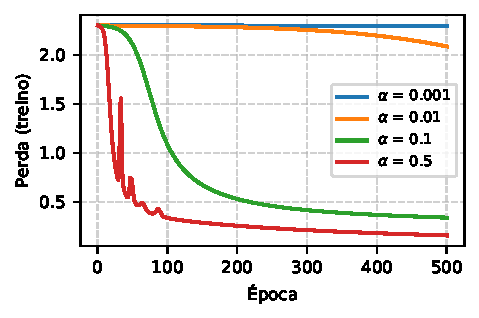
\includegraphics[width=\columnwidth]{figures/fig_taxa.pdf}
\caption{Perda de treino por época para cada taxa de aprendizado ($H = 64$).}
\label{fig:taxa}
\end{figure}

\begin{figure}[t]
\centering
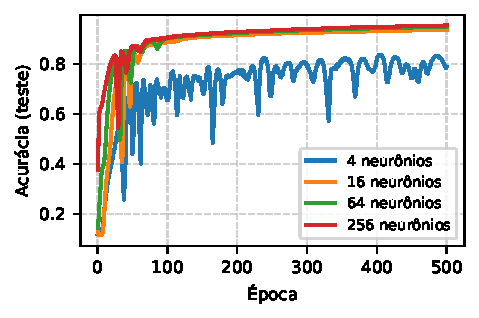
\includegraphics[width=\columnwidth]{figures/fig_neuronios.pdf}
\caption{Acurácia de teste por época para cada número de neurônios ($\alpha = 0{,}5$).}
\label{fig:neuronios}
\end{figure}

\subsection{Taxa de Aprendizado}
Com $\alpha = 0{,}001$ a perda não sai de $\ln 10 \approx 2{,}30$ (o chute uniforme) em 500 épocas, e com $0{,}01$ só chega a 2,09 (Tabela~\ref{tab:resultados} e Figura~\ref{fig:taxa}): os passos são curtos demais. A partir de $0{,}1$ a acurácia passa de 90\%, e $0{,}5$ é a melhor taxa (94,96\%). Sua curva, porém, tem picos de perda nas primeiras $\sim$100 épocas (o maior perto da época 30, de 0,73 para 1,56): passos grandes demais fazem a rede ultrapassar o mínimo antes de se acomodar.

\subsection{Número de Neurônios}
A acurácia cresce com $H$, com retornos decrescentes (Figura~\ref{fig:neuronios}): de 4 para 16 neurônios ganha quase 15 pontos, e de 64 para 256 só 0,5 ponto, por 2,9 vezes o tempo. Com 4 neurônios e $\alpha = 0{,}5$, a acurácia oscila entre cerca de 50\% e 84\% até o fim e termina abaixo do pico (78,8\% contra 83,7\%): pouca capacidade e uma taxa grande demais para ela.

\subsection{Número de Épocas}
Com 100 épocas a acurácia já passa de 90\%, e de 200 para 500 o ganho é de 2,5 pontos. Com semente fixa e lote completo o treino é determinístico, então o treino de 50 épocas é idêntico às primeiras 50 épocas do de 500. Com 50 épocas, a acurácia final (78,8\%) fica abaixo do pico do próprio treino (85,2\%): o treino para dentro da fase instável, logo após um pico de perda.

\subsection{Melhor Configuração}
Com $\alpha = 0{,}5$, $H = 256$ e 500 épocas, a perda final foi 0,1462 e a acurácia de teste, 95,44\%, em 283\,s; ao fim, as curvas ainda melhoram, então mais épocas trariam algum ganho. Por dígito, os mais fáceis são 1 (97,8\%), 0 e 6 (97,5\%) e os mais difíceis, 8 (93,2\%) e 9 (93,5\%). As maiores confusões são 4$\to$9 (37 imagens), 9$\to$4 (32), 5$\to$3 (28), 8$\to$3 (26), 3$\to$5 (23) e 9$\to$7 (20). Para comparar, o primeiro treino pela interface ($\alpha = 0{,}01$, $H = 8$, 10.000 épocas, cerca de 15 min) chegou a 90,63\%.

\subsection{Testes na Interface}
Desenhando livremente, o desempenho ficou bem abaixo dos 95\%. A rede teve mais facilidade com o 4 e, especialmente, com o 2; nos demais dígitos, acertar dependeu de entender onde desenhar o número. Sem esse ajuste, o modelo quase nunca acertou o 8 e o 9, que também são os piores dígitos no teste. Quando peguei o jeito de desenhar com o centro de massa onde a rede esperava, perto do centro da grade como no MNIST, o desempenho ficou mais satisfatório.

No caso da Figura~\ref{fig:deslocamento}, o centro de massa do ``1'' desenhado ficou em (11,9; 11,7), contra (14; 14) no MNIST, e a rede respondeu 8 (52\%); o mesmo desenho deslocado 2 pixels virou 1 (99\%). O efeito se generaliza: deslocar todas as imagens de teste 2 pixels para a direita derruba a acurácia de 95\% para 71\%, e mais neurônios não resolvem (as redes de 64 e 256 neurônios empatam em 71,3\%).

\begin{figure}[h]
\centering
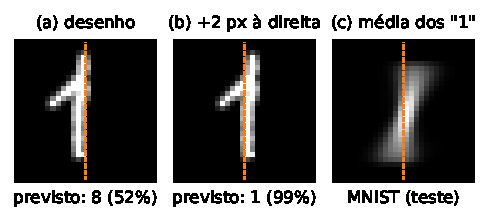
\includegraphics[width=\columnwidth]{figures/fig_deslocamento.pdf}
\caption{Um ``1'' desenhado na interface (a), o mesmo desenho deslocado 2 pixels para a direita (b) e a média dos ``1'' do conjunto de teste (c), com a previsão da melhor rede. A linha tracejada marca a coluna central.}
\label{fig:deslocamento}
\end{figure}

% ---------------------------------------------------------------------------
\section{Discussão}
\textbf{Trade-offs.} Taxas pequenas são estáveis, mas não saem do lugar em 500 épocas; 0,5 converge rápido, mas oscila no começo e desestabiliza redes pequenas. Já o custo por época cresce com $H$ (com o lote completo, a matriz de 56.000 $\times$ 784 é multiplicada duas vezes por época), enquanto o ganho de acurácia satura.

\textbf{Por que o desenho falha.} O MNIST é padronizado: cada dígito foi redimensionado para uma caixa de 20$\times$20 e centralizado pelo centro de massa \citep{lecun1998gradient}, e a interface envia os pixels do canvas sem esse tratamento. Numa rede totalmente conectada, cada peso de $W_1$ está preso a um pixel fixo, então a rede não tem invariância a translação; \citet{lecun1998gradient} apontam essa como a principal deficiência dessas redes para imagens e a motivação das redes convolucionais, que replicam os pesos ao longo da imagem. Os 95\% valem para imagens com a mesma distribuição do treino, e o desenho livre vem de outra. É um exemplo de como a acurácia e a perda podem enganar quando o conjunto de teste não representa a realidade como um todo: com essa sensibilidade a poucos pixels, o modelo é quase inutilizável na prática. As confusões (4/9, 3/5/8, 7/9) seguem a mesma lógica: são dígitos que diferem em poucos pixels, como um traço fechado ou aberto.

\textbf{Limitações.} Gradiente em lote completo (lento por época), uma camada escondida, uma única semente por configuração (diferenças de meio ponto podem ser ruído), busca coordenada em vez de grade completa e escolha da melhor configuração pelo próprio conjunto de teste, sem validação separada.

% ---------------------------------------------------------------------------
\section{Conclusão}
Funcionaram melhor uma taxa de aprendizado alta e mais neurônios, com 95,44\% de acurácia; a taxa foi decisiva para o tempo de treino, já que a melhor rede superou em 5 minutos um treino de 15 minutos pela interface. Como melhorias: pré-processar o desenho como o MNIST (recorte, redimensionamento e centralização pelo centro de massa), aumentar os dados com deslocamentos, usar minilotes e usar redes convolucionais, que compartilham os pesos no espaço e por isso toleram deslocamentos.

% ---------------------------------------------------------------------------
\section{Declaração de Uso de IA}
Foi usado o Claude Code (modelo Claude Opus 5.5, da Anthropic) para: explicar conceitos e NumPy (softmax e estabilidade numérica, \texttt{axis}, \texttt{keepdims}, \emph{broadcasting}, entropia cruzada); validar as funções contra os resultados esperados do enunciado; depurar o salvamento dos pesos e recuperar o primeiro treino; analisar o desenho mal classificado; gerar os scripts auxiliares de experimentos e de figuras; pesquisar a referência sobre invariância a translação; escrever o README do repositório; e montar o esqueleto deste relatório, contendo as tabelas. O texto final foi redigido e escrito por mim, assim como as funções do \texttt{learn.py}. Transcrições: \url{https://github.com/Vipigal/mnist-neural-network-training/blob/main/uso-de-ia/conversa-claude-code.md}.

\bibliography{referencias}

\end{document}
